\documentclass[serif,9pt]{beamer}
\usepackage{color,listings}
\usepackage{ragged2e}
\usepackage[spanish]{babel}
\usepackage{graphicx}

\definecolor{dkgreen}{rgb}{0,0.6,0}
\definecolor{gray}{rgb}{0.5,0.5,0.5}
\definecolor{mauve}{rgb}{0.58,0,0.82}
\definecolor{lgray}{rgb}{0.99,0.97,0.95}
\newcommand{\X}{\textbf{X}}
\newcommand{\Y}{\textbf{Y}}
\newcommand{\Z}{\textbf{Z}}
\newcommand{\G}{\textbf{G}}
\newcommand{\R}{\textbf{R}}
\newcommand{\V}{\textbf{V}}
\newcommand{\Q}{\textbf{Q}}
\newcommand{\h}{\textbf{H}}
\newcommand{\T}{\textbf{T}}

\def\E{\mathbb{E}}
\def\C{\mathbb{C}}
\def\N{\mathbb{N}}


\usetheme{Frankfurt}
%\usecolortheme{rose}
\usecolortheme{lily}
\usepackage{amsmath, multirow}
%\usepackage{color, amsmath, wrapfig, anysize, graphicx, hyperref, amsthm, fancyhdr, amssymb,geometry,amsfonts,float}

\newcommand{\ds}{\displaystyle}


\titlegraphic{
\includegraphics[width=4cm]{utfsm.eps}}%
   %\includegraphics[width=4cm]{fig/inria.eps}}

\begin{document}
\title[Una Arquitectura de Referencia para Web
Browsers]{Hacia una unificaci\'on de Conceptos de Seguridad} 
\author[Paulina Silva Ghio]{\textsc{Paulina Silva Ghio} \\ \medskip
\small{}
Departamento de Inform\'atica - UTFSM\\ \medskip
\url{pasilva@alumnos.inf.utfsm.cl}}
\institute[]{}
\date{24-11-2015.}

\begin{frame}[plain]
\titlepage
\end{frame}


\begin{frame}
\frametitle{Indice}
\tableofcontents
\end{frame} 


\section{Introducci\'on}
\subsection{Contexto}
\begin{frame}
\frametitle{Contexto}

	\begin{itemize}
		\item La guerra de los Navegadores: construir y parchar.
		\item El navegador web: herramienta de uso cotidiano.
		\item El usuario com\'un utiliza servicios.
		\item Distintos tipos, distintas implementaciones.
		\item Web 2.0 y 3.0: AJAX (Asynchronous Javascript and XML).
	\end{itemize}
\end{frame}


\begin{frame}
\frametitle{Browser en la Actualidad}
	\begin{figure}[h]
	    \centering
	    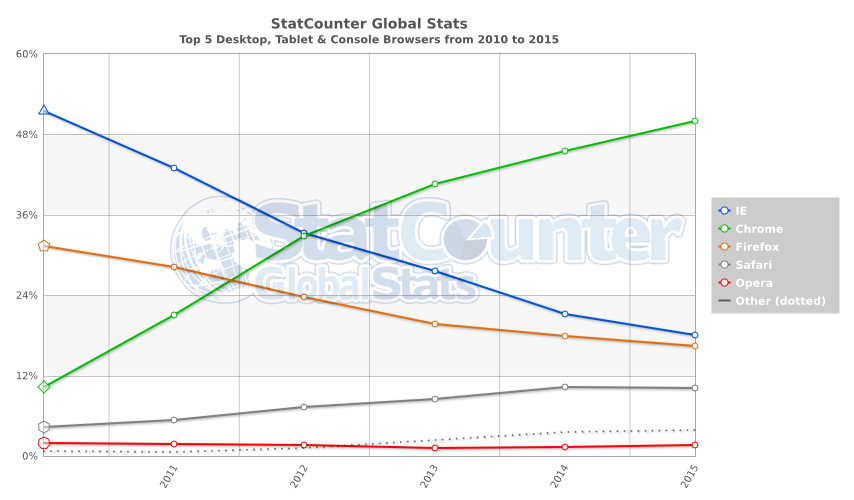
\includegraphics[width=1\textwidth]{figures/StatCounter-browser-ww-yearly-2010-2015.png}
	    \caption{Porcentaje de uso de Navegadores. Fuente: \cite{statBrow}}
	    \label{fig:UsageShare}
	\end{figure}
\end{frame}


\subsection{Seguridad...}
\begin{frame}
\frametitle{Seguridad...}
	\begin{block}{Desde la perspectiva de seguridad \cite{WhyteHarrison}:}
		\begin{itemize}		
			\item �Qu\'e realizan las universidades o la industria respecto a estas preocupaciones?
			\item Projectos de desarrollo de software, �cuanto se le dedica a la seguridad?
		\end{itemize}
	\end{block}
	\begin{block}{�Qu\'e conceptos de seguridad sabe en promedio un estudiante graduado de carrera relacionada a Computer Science?}
		\begin{itemize}
			\item �La gente es autodidacta? o �aprende por necesidad?
			\item �La malla curricular es suficiente?
			\item �La industria asegura que los sistemas a construir, sean seguros?
		\end{itemize}
	\end{block}
\end{frame}



\subsection{Desarrollo de Software y Seguridad}
\begin{frame}
\frametitle{Desarrollo de Software y Seguridad}
	\begin{itemize}
		\item �Qu\'e tanto se diferencian las preocupaciones del usuario com\'un y el desarrollador que crea los sistemas?
		\item �C\'omo desarrollar software seguro?
	\end{itemize}
	\begin{block}{Construcci\'on de Software Seguro...}
		\begin{itemize}
			\item Los que participan en la construcci\'on: deben entender los problemas de seguridad.
			\item No basta saber como est\'a construido.
			\item Considerar la Seguridad desde el inicio del Proyecto.
			\item Seguridad como una Propiedad Sist\'emica.
		\end{itemize}
	\end{block}
\end{frame}

\subsection{Motivaci\'on para estudiar este tema}
\begin{frame}
	\frametitle{Motivaci\'on}
	\begin{itemize}
		\item Nuevas formas de interactuar.
		\item Permite disminuir los costos de construir un programa Cliente (desde cero) para
el usuario del sistema.
		\item Seguridad implementada que los Web Browser es bastante buena.
		\item El browser es una herramienta indispensable.
	\end{itemize}

	\begin{block}{Las preocupaciones principales}
	\begin{itemize}
		\item Los sistemas, a los que un usuario hace referencia, son llamados desde un Web Browser.
		\item El stakeholder afectado: el usuario del Browser, el Host del usuario y hasta el Servicio externo usado.
		\item Falta de conocimientos de seguridad con respecto al Browser, podr\'ia afectar de forma directa el desarrollo de aplicaciones que lo utilizan.
	\end{itemize}

	\end{block}
\end{frame}

\subsection{Contribuciones}
\begin{frame}
	\frametitle{Contribuciones}
	\begin{block}{Objetivo General}
		\begin{itemize}
			\item Generar un cuerpo organizado de informaci\'on sobre el Web Browser y su seguridad, de tal manera que se pueda sistematizar, organizar y clasificar el conocimiento adquirido en un documento, con formato semi-formal, tanto para Profesionales como Estudiantes del \'area Inform\'atica que est\'en insertos en el \'area de Desarrollo de Software.
		\end{itemize}
	\end{block}
\end{frame}

\begin{frame}
	\frametitle{Contribuciones}
	\begin{block}{Objetivos Espec\'ificos}
		\begin{itemize}
			\item Comprender los conceptos relacionados al navegador web, sus componentes, interacciones o formas de comunicaci\'on, amenazas y ataques a los que puede estar sometido, como tambi\'en los mecanismos de defensa. Esto se realizar\'a a trav\'es del desarrollo de un Estado del Arte sobre el Browser.
			\item Identificar actores, componentes, funciones, relaciones, requerimientos y restricciones del navegador, para lograr abstraer una Arquitectura de Referencia (AR) a partir de documentaci\'on disponible en Internet, blogs de desarrolladores, papers e iniciar un peque�o cat\'alogo de Patrones de Mal Uso. Esto permitir\'a condensar el conocimiento obtenido en el punto anterior a trav\'es de documentos semi-formales, lo que permitir\'a generar una gu\'ia para comunicar los conceptos relevantes que pudieran afectar la relaci\'on existente entre un desarrollo de software y el navegador.
			\item Profundizar el conocimiento en ataques relacionados con m\'etodos de Ingenier\'ia Social
		\end{itemize}
	\end{block}
\end{frame}

\section{Marco Te\'orico de un Browser}
\begin{frame}
	\frametitle{Marco Te\'orico de un Browser}
	\begin{itemize}
		\item Arquitectura cliente/servidor
		\item Comunicaci\'on e Informaci\'on de estado: HTTP y canales.
		\item SSL/TLS
		\item HTML5 y XML (Markup Languages)
		\item CSS
		\item DOM
		\item Javascript (ECMAScript)
		\item Geolocalizaci\'on, WebWorkers y otros...
	\end{itemize}
	\begin{block}{Desaf\'ios del navegador}
		\begin{itemize}
			\item Contenido y compatibilidad
			\item Navegaci\'on personalizada
			\item Navegaci\'on sin inconvenientes
			\item Seguridad
		\end{itemize}
	\end{block}
\end{frame}


\begin{frame}
	\frametitle{Arquitectura de Referencia (AR) y Patrones de Mal Uso}
	\begin{block}{AR}
		\begin{itemize}
			\item Especifica la decomposici\'on del sistema en subsistemas, las interacciones entre estas partes y la distribuci\'on de funcionalidad entre ellas.
			\item Capturar la esencia de la arquitectura a trav\'es de una colecci\'on de sistemas similares, por medio del reuso arquitect\'onico
			\item Ayudar a los implementors o desarrolladores del software, a entender los trade-off cuando se dise�an nuevos sistemas
			\item Ayudar a los mantenedores de estos sistemas a entender el c\'odigo legacy usado.
			\item Comparar las diferencias en decisiones de dise�o y poder entender los cambios realizados a lo largo del Desarrollo de un sistema.
			\item Mirada hol\'istica del Sistema.
		\end{itemize}
	\end{block}
	\begin{block}{Patrones del Mal Uso}
		\begin{itemize}
			\item Permitir\'an ense�ar y comunicar las posibles formas en que tal sistema puede ser usado inapropiadamente.
		\end{itemize}
	\end{block}
\end{frame}

\begin{frame}
	\frametitle{Arquitectura de Referencia (AR)}
	\begin{itemize}
		\item Describir los Stakeholders que interactuan con el sistema y que poseen preocu paciones/concerns de \'este.
		\item Patrones de Arquitectura.
		\item Atributos de calidad deseables que el sistema debe garantizar. Es importante solo destacar aquellos realmente necesarios, dado que un sistema sobrecargado con ellos tampoco es conveniente.
	\end{itemize}
	\begin{block}{Ventajas}
		\begin{itemize}
			\item Comprender la estructura subyacente de un Web Browser y las interacciones que tendr\'a con otros sistemas.
			\item Proveer una base tecnol\'ogica modular y flexible. Al tener los subsistemas compartimentalizados es posible quitar y sacar piezas, que poseen interfaces similares, y de esa manera reusar lo otro sin tener que construir un sistema nuevo.
			\item Entrega una base para el desarrollo de otros Navegadores Web, sin explicar detalles de implementaci\'on.
		\end{itemize}
	\end{block}
\end{frame}

\section{(In)Seguridad en el Browser}
\begin{frame}
	\frametitle{Ataques y Amenazas}
	\begin{itemize}
		\item Social Engineering Attacks o Ataques de Ingenier\'ia Social: Phishing
		\item Instalaci\'on de Malware o extensiones malignas
		\item Extensiones Vulnerables
		\item Ejecuci\'on de c\'odigo Javascript
		\item XSS-DOM
		\item Man-in-the-Browser
	\end{itemize}
\end{frame}

\subsection{Mecanismos de Defensa}
\begin{frame}
	\frametitle{Ataques y Amenazas}
	\begin{itemize}
		\item SOP o Same Origin Policy
		\item CORS o Cross-Origin Resource Sharing
		\item HTTP Fields o Campos HTTP
		\item Sandboxing: Google Chrome/Chromium e Internet Explorer
		\item Aislaci\'on de Contenido
		\item Blacklist y Whitelist
		\item Sistema de Reputaci\'on
		\item Actualizaciones peri\'odicas en background
	\end{itemize}
\end{frame}


\section{Estado del Arte}
\begin{frame}
	\frametitle{Estado del Arte}
	\begin{itemize}
		\item No se encontr\'o informaci\'on actualizada sobre una Arquitectura de Referencia del Browser. Hay una \cite{preprint-grosskurth-browser-archevol}, pero es muy antigua.
		\item Poca documentaci\'on y no hay conceptos unificados.
	\end{itemize}
	\begin{figure}[h]
	    \centering
	    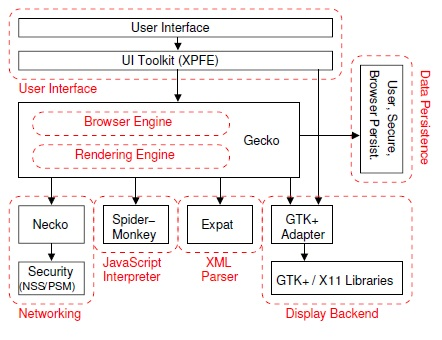
\includegraphics[scale=0.5]{figures/archMoz.jpg}
	    \caption{Arquitectura de Browser monoproceso. Fuente: \cite{preprint-grosskurth-browser-archevol}}
	    \label{fig:armonoproceso}
	\end{figure}
\end{frame}

\subsection{Google Chrome y Chromium}
\begin{frame}
	\frametitle{Google Chrome y Chromium}
	\begin{figure}[h]
	    \centering
	    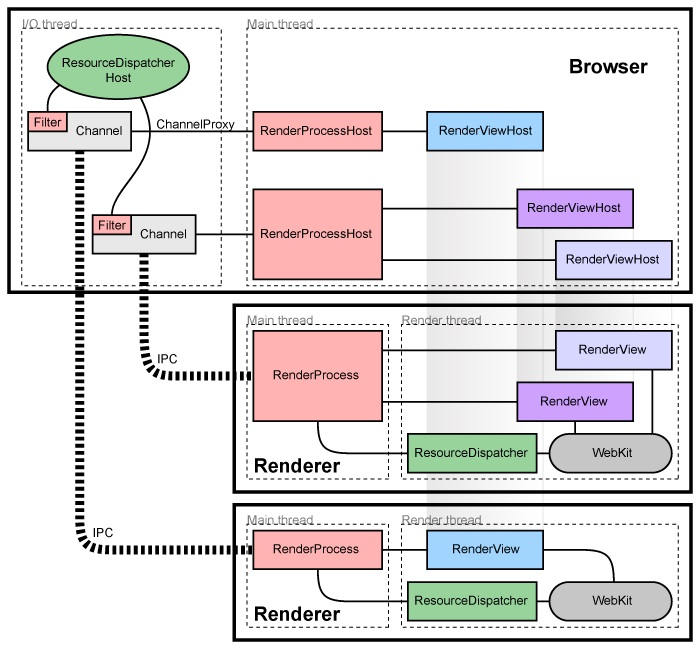
\includegraphics[scale=0.35]{figures/archGC.jpg}
	    \caption{Architectura Multiprocesos de Google Chrome. Fuente: \cite{multiProcGC}}
	    \label{fig:UsageShare}
	\end{figure}
\end{frame}

\begin{frame}
	\frametitle{Google Chrome y Chromium}
	\begin{figure}[h]
        \centering
        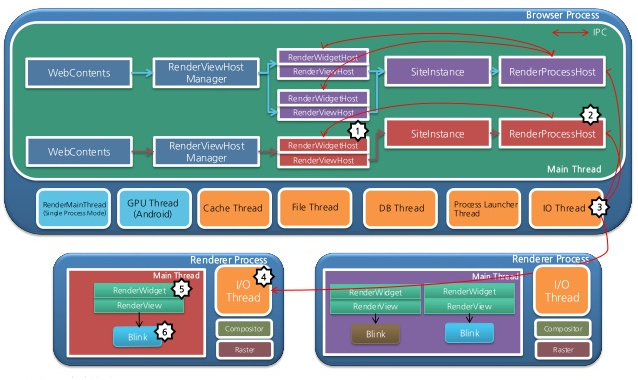
\includegraphics[scale=0.4]{figures/chromium-rendering-pipeline-28-638.jpg}
        \caption{Architectura de Chromium en detalle. Fuente: \cite{ChrRenderPipe}}
        \label{fig:archGC2}
    \end{figure}
\end{frame}

\subsection{Internet Explorer}
\begin{frame}
	\frametitle{Internet Explorer}
	\begin{figure}[h]
	    \centering
		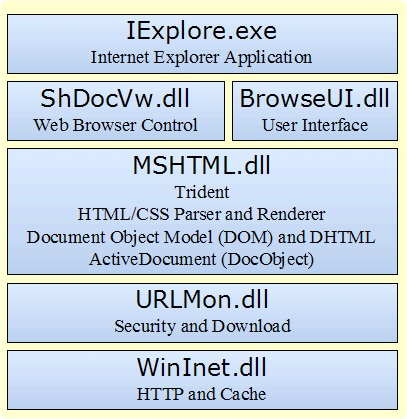
\includegraphics[scale=0.5]{figures/IEArch.jpg}
		\caption{Arquitectura de Internet Explorer. Fuente: \cite{IEArchImg}}
		\label{fig:archIE}
    \end{figure}
\end{frame}

\begin{frame}
	\frametitle{Internet Explorer}
	\begin{figure}[h]
        \centering
        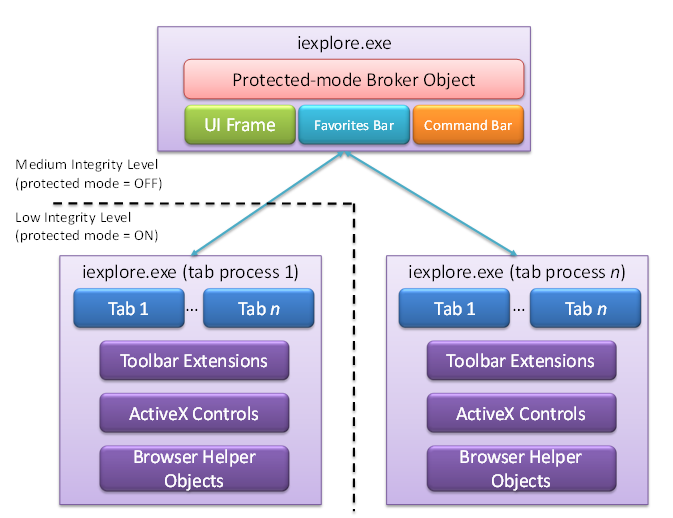
\includegraphics[scale=0.35]{figures/11_IE8andLooselyCoupledIELCIE_2.png}
        \caption{Arquitectura de Internet Explorer m\'as detallada. Fuente: \cite{IE8LCIE}}
        \label{fig:archIE2}
    \end{figure}
\end{frame}

\subsection{Firefox - Electrolysis}
\begin{frame}
	\frametitle{Firefox - Electrolysis}
	\begin{figure}[h!t]
        \centering
        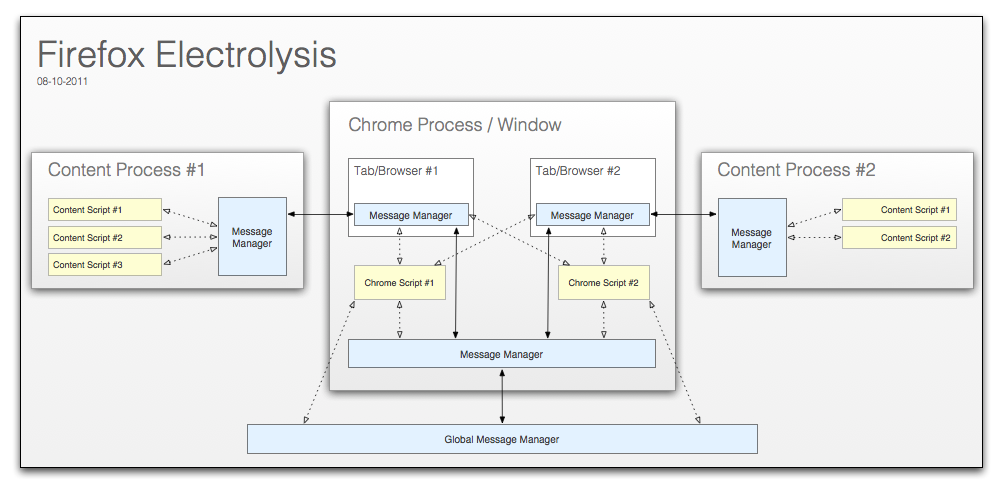
\includegraphics[scale=0.3]{figures/electrolysis.png}
        \caption{Firefox Electrolysis, Comunicaci\'on de procesos 1. Fuente: \cite{Firefox101}}
        \label{fig:ChromePComm1}
    \end{figure}
\end{frame}

\begin{frame}
	\frametitle{Firefox - Electrolysis}
	\begin{figure}[h!t]
        \centering
        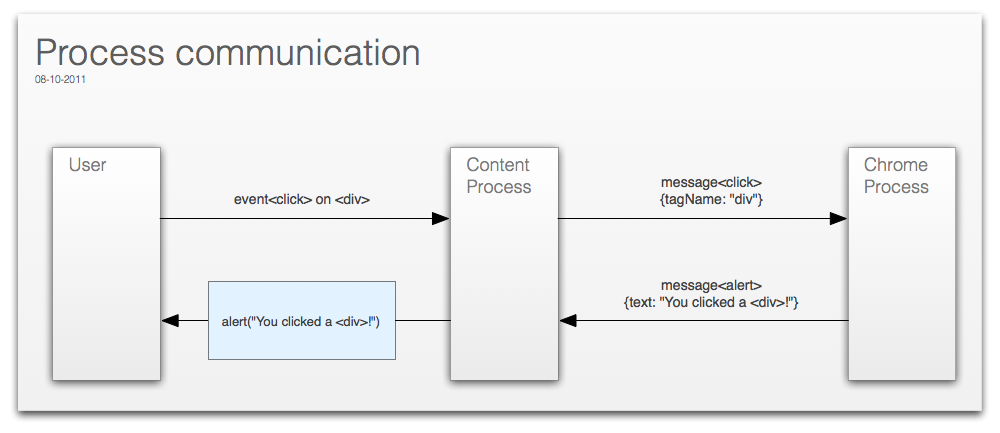
\includegraphics[width=1\textwidth]{figures/e10s-processes.png}
        \caption{Firefox Electrolysis, Comunicaci\'on de procesos 2. Fuente: \cite{Firefox101}}
        \label{fig:ChromePComm2}
    \end{figure}
\end{frame}

\section{Arquitectura de Referencia}
\begin{frame}
	\frametitle{Casos de Uso}
	\begin{figure}[h]
	    \centering
	    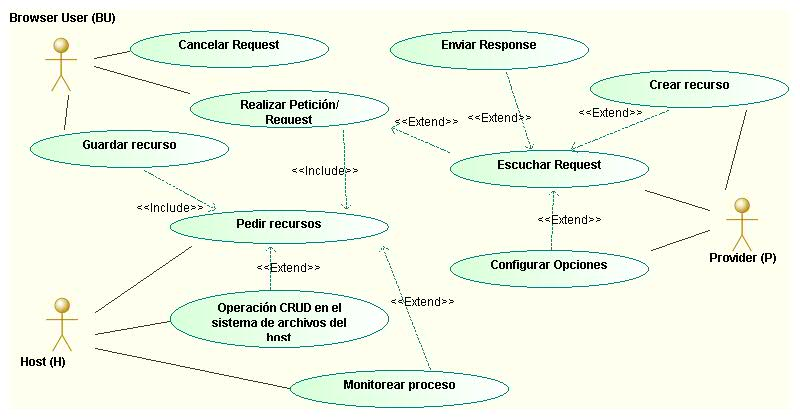
\includegraphics[scale=0.35]{figures/chap4/UCBrowser.jpg}
	    \caption{Diagrama de Caso de Uso del \textit{Web Browser}.}
	    \label{fig:CUBrowser}
	\end{figure}
\end{frame}

\begin{frame}
	\frametitle{Patr�n Browser Infrastructure}
	\begin{figure}[h]
	    \centering
	    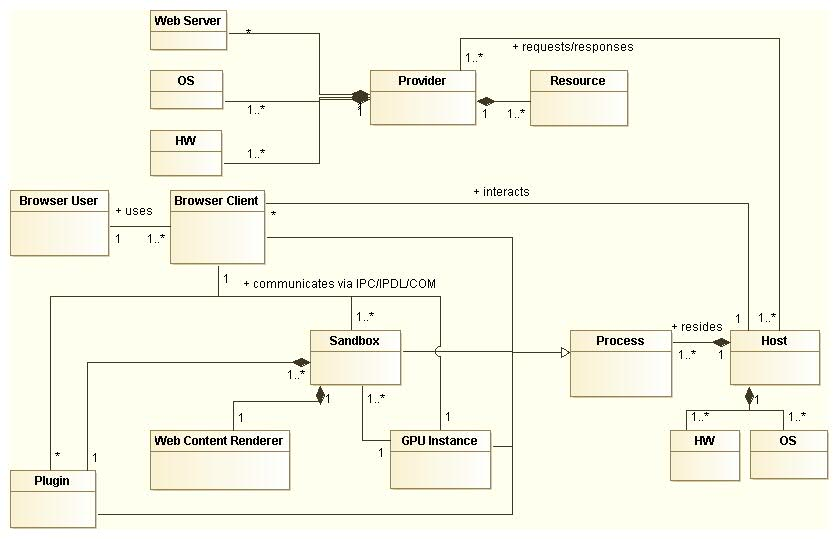
\includegraphics[scale=0.35]{figures/chap4/browserInfraPattern_v3.jpg}
	    \caption{Componentes de alto nivel del \textit{Browser}.}
	    \label{fig:BIPatt}
	\end{figure}
\end{frame}


\begin{frame}
	\frametitle{Din�mica: Realizar Request}
	\begin{figure}[h]
	    \centering
	    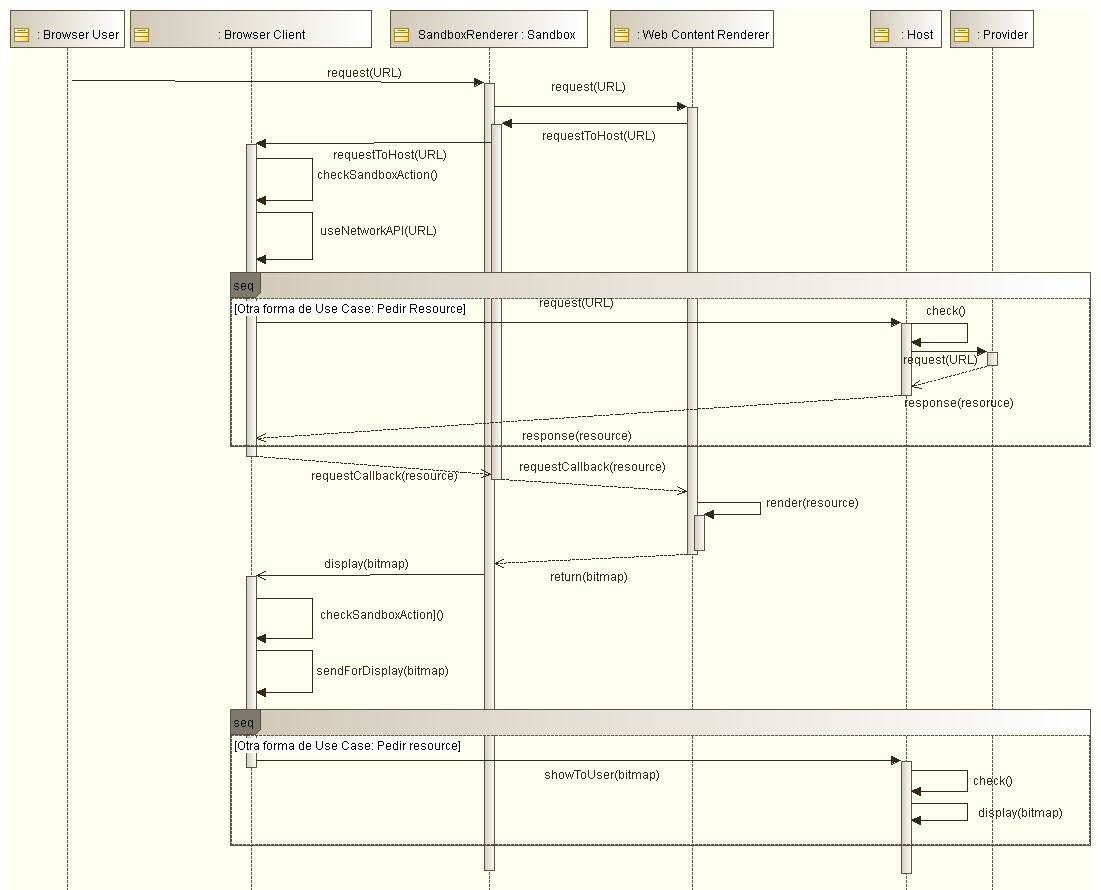
\includegraphics[scale=0.28]{figures/chap4/requestResource_v2.jpg}
	    \caption{Diagrama de Secuencia: Realizar Request.}
	    \label{fig:SecReq}
	\end{figure}
\end{frame}

\section{Patr�n de Mal Uso}
\begin{frame}
	\frametitle{Diagrama de Actividad}
	\begin{figure}[h]
	    \centering
	    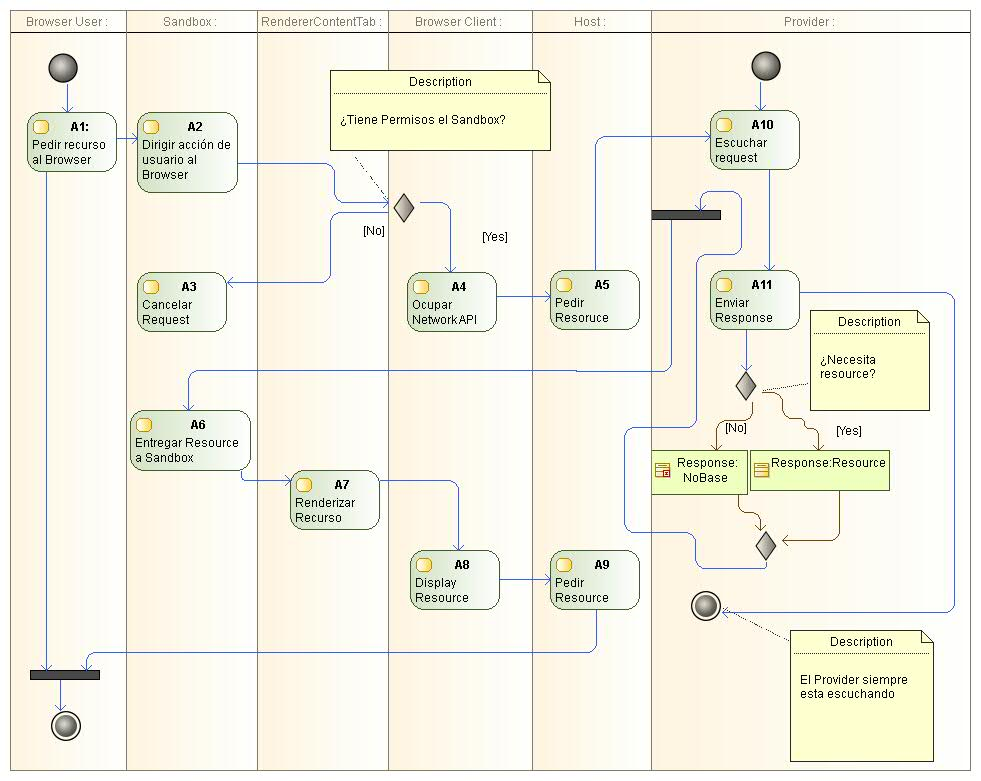
\includegraphics[scale=0.23]{figures/chap5/activityDiag_v3.jpg}
	    \caption{Diagrama de Actividad Compuesto para los casos de uso \textbf{Realizar Request} y \textbf{Recibir Request}.}
	    \label{fig:ActDiagr}
	\end{figure}
\end{frame}

\begin{frame}
	\frametitle{Diagrama de Clases para el patr�n de Mal Uso.}
	\begin{figure}[h]
	    \centering
	    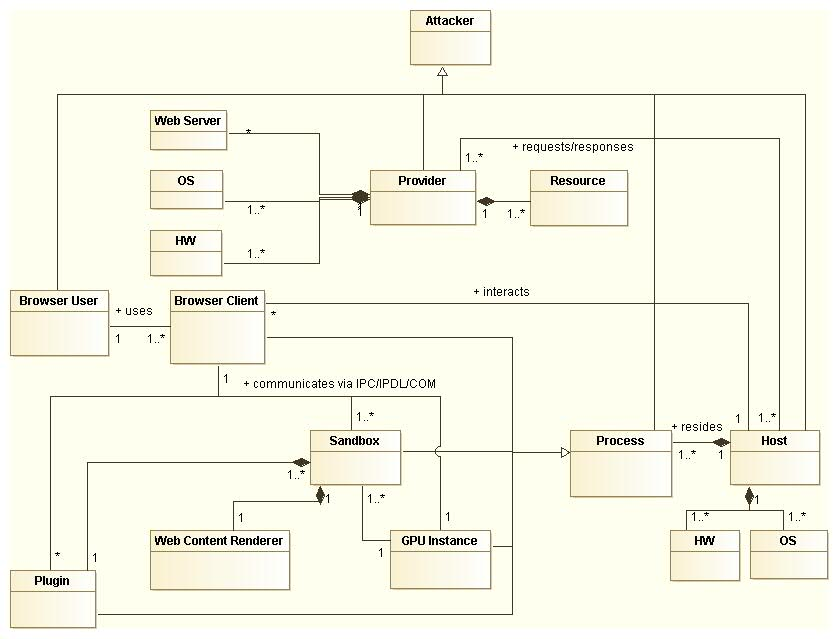
\includegraphics[scale=0.3]{figures/chap5/patronMisuse_v2.jpg}
	    \caption{Diagrama de Clases para el patr�n de Misuse.}
	    \label{fig:BIMisuse}
	\end{figure}
\end{frame}

\begin{frame}
	\frametitle{Diagrama de Clases para el patr�n de Mal Uso.}
	\begin{figure}[h]
        \centering
        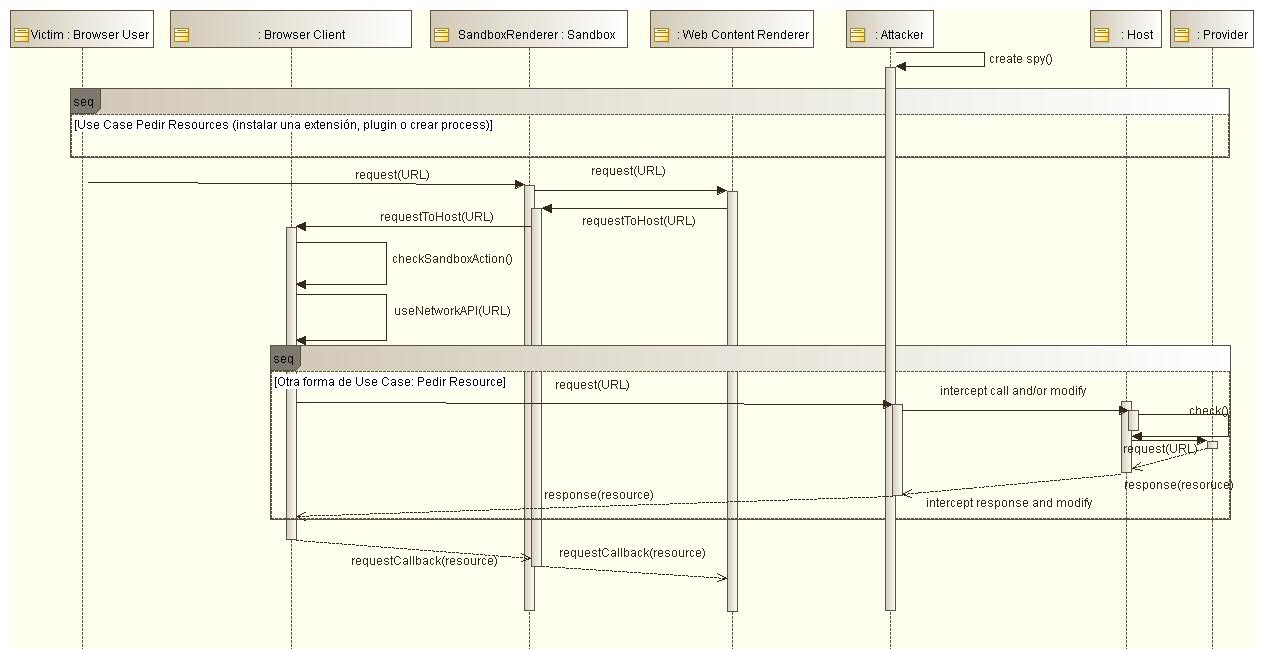
\includegraphics[scale=0.32]{figures/chap5/patronMisuseSeq_v2.jpg}
        \caption{Diagrama de Secuencia para el Mal uso: Modificaci�n de tr�fico en el \textit{Web Browser}.}
        \label{fig:SeqMisuse}
    \end{figure}
\end{frame}


\section{Conclusiones}
\begin{frame}
	\frametitle{Conclusiones}
\end{frame}


\bibliography{refTodas}
\bibliographystyle{IEEEtran}

\end{document}

